\section{Class 9 - 26/03/21}
In today's class we will go on with antennas: starting again with the Hertzian dipole, and how it irradiates on space
\subsection*{Hertzian Dipole useful parameters}
It is useful to look at some dipole parameters, because them are simple to understand, and then we can generalize those for other types of antenna.
\subsubsection*{Hertzian Dipole radiation pattern}
The aim of this section is to find out the radiation pattern of a little Hertzian antenna.\\
First of all, we need to remember that the radiation pattern is a "representation" of the radiation function $f(\theta,\varphi)=\sqrt{i_r(\theta,\varphi)}$.\\
That being said, we need to calculate the radiation intensity: we need to apply it's definition in \cref{eq:radiation_intensity} with the well known electric field of the Hertzian dipole in \cref{eq:EMF_components_in_spherical_2}:
\begin{equation}\label{eq:radiation_intensity2}
    I_r(\theta, \varphi)=\frac{|E(\theta,\varphi)|^2}{2\eta}=\frac{\eta}{8}\left(\frac{d}{\lambda}\right)^2I_0^2\,\sin^2(\theta)
\end{equation}
The only thing that can change in \cref{eq:radiation_intensity2} is the $\sin^2(\theta)$, so finding the maximum value of radiation intensity is a simple task: we just need to let the $\sin(\theta)$ value to be equal to $1$.\\
Then the normalized radiation intensity becomes:
\begin{equation}\label{eq:normalized_rad_intensity}
    i_r=\frac{I_r}{I_r^{max}}=\sin^2(\theta)
\end{equation}
And the radiation function:
\begin{equation}
    f(\theta,\varphi)=\sqrt{i_r(\theta,\varphi)}=|\sin(\theta)|
\end{equation}
Now that we have $f(\theta, \varphi)$ we need think about how to plot it in a 3d plot. We will use the spherical coordinate that we saw in \cref{fig:3d_plot}.\\
We could give this $f$ function to a 3-d calculator, and the figure will pop out in few seconds, but if we want to know better how this is made, we could imagine to slice our plot in the various plane, then we merge them and we obtain the full 3d plot.\\
First of all we see our function in the (x,z) plane: here we can move by varying the $\theta$ angle, and then the equation for the 2d plot in this plane are:
\begin{equation}
    \begin{cases}
        x=f\,\sin(\theta)=|\sin(\theta)|\,\sin(\theta)\\[5pt]
        z=f\,\cos(\theta)=|\sin(\theta)|\,\cos(\theta)
    \end{cases}\label{eq:x-z_equation}
\end{equation}
If we plot the system in \cref{eq:x-z_equation}, we will obtain a curve with two adjacent circles, like an overturned $8$. It is more simple to see it in \cref{fig:Dipolexz}
\begin{figure}[H]
    \begin{center}
        \begin{tikzpicture}
            \begin{polaraxis}[axis lines = none]
                \addplot[domain=0:360,samples=73,smooth] (x+90,{abs(sin(x))});
            \end{polaraxis}
            \draw[-stealth] ([yshift=1.5cm]current axis.south) -- ([yshift=-1.5cm]current axis.north) node[anchor=north,yshift=1cm]{$z$};
            \draw[-stealth] (current axis.west) -- (current axis.east) node[anchor=west]{$x$};
        \end{tikzpicture}
        \caption{Hertzian dipole radiation pattern in x-z plane}\label{fig:Dipolexz}
    \end{center}
\end{figure}
We can notice that $f$ is not dependent on $\varphi$, and this simplify our job because in the (x,y) plan we will obtain a circumference. Remember that in the y-x plan the only parameter that change is $\varphi$, so for a given $\theta$ and $r$ we will draw semi-circumference moving $\varphi$ from $0$ to $2\phi$. In you can see this x-y plot.
\begin{figure}[H]
    \begin{center}
        \begin{tikzpicture}
            \begin{polaraxis}[axis lines = none]
                \addplot[domain=0:360,samples=73,smooth] (x+90,1);
            \end{polaraxis}
            \draw[-stealth] (current axis.south) -- (current axis.north) node[anchor=north,yshift=1cm]{$y$};
            \draw[-stealth] (current axis.west) -- (current axis.east) node[anchor=west]{$x$};
        \end{tikzpicture}
        \caption{Hertzian dipole radiation pattern in x-y plane}\label{fig:Dipolexy}
    \end{center}
\end{figure}
At the end, if we merge the information that we have collected until now, we can plot the 3 dimensional plot of our radiation pattern.\\
In \cref{fig:3dplot_radiation_dipole} you can see a colorful example of dipole radiation pattern (the colours have no mean, they simply change with $\theta$ because it looks good imo)

\begin{comment}
\begin{figure}[H]\begin{center}
    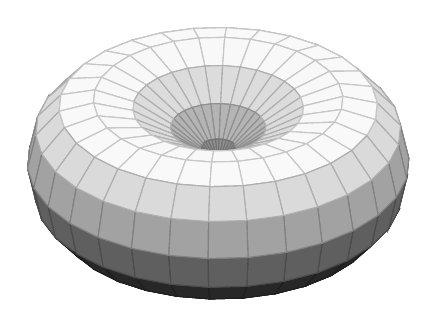
\begin{tikzpicture}
    \begin{axis}[view/h=45,axis lines = none,
            unit vector ratio=1 1 1]
            \addplot3[domain=0:360,domain y=0:360,samples=31,
            colormap/blackwhite,surf,%mesh,point meta=1, %<-if you want a mesh
            z buffer=sort
            ]
           ({(sin(x+90)*sin(x+90))*cos(y)}, 
            {(sin(x+90)*sin(x+90))*sin(y)}, 
            {(sin(x+90)*sin(x+90))*sin(x)});
    \end{axis}
    \end{tikzpicture}\caption{3d plot}\label{fig:3dplot}
\end{center}
\end{figure}
\end{comment}

\tdplotsetmaincoords{70}{135}
\begin{figure}[H]\begin{center}
    \begin{tikzpicture}[scale=2,line join=bevel,tdplot_main_coords, fill opacity=.7]
        \pgfsetlinewidth{.4pt}
        \tdplotsphericalsurfaceplot[parametricfill]{72}{24}%
        {abs(sin(\tdplottheta))}{black}{\tdplotphi}%
        {\draw[color=black,thick,->] (0,0,0) -- (2,0,0) node[anchor=north east]{$x$};}%
        {\draw[color=black,thick,->] (0,0,0) -- (0,2,0) node[anchor=north west]{$y$};}%
        {\draw[color=black,thick,->] (0,0,0) -- (0,0,1) node[anchor=south]{$z$};}
    \end{tikzpicture}
    \end{center}\caption{Hertzian dipole radiation pattern 3d}\label{fig:3dplot_radiation_dipole}
\end{figure}
\subsection*{$R_{in}$ of an Hertzian dipole}
As we have already seen in \cref{fig:impedance_antenna}, our antenna could be seen like a bunch of impedance in series, and we could be interested in calculating one of them, like $R_{in}$.
From the definition of the emitted power in \cref{eq:emitted_power2} we can obtain:
\begin{equation}
    P_a=\frac{1}{2}R_in\,|I_0|^2=\frac{\eta \pi}{3}\left(\frac{d}{\lambda}\right)^2I_0\,\rightarrow \bf{R_{in}} =\frac{2}{3}\eta\pi\left(\frac{d}{\lambda}\right)^2
\end{equation}
\subsubsection*{Directivity of an Hertzian dipole}
It is interesting to see the directivity of the Hertzian dipole, and it will be very poor (as expected):
\begin{align}\label{eq:directivity_hertzian_dipole}
    \begin{split}
        D&=\frac{1}{\frac{1}{4\pi \int_{4\pi}i_r\,d\Omega}}=\\[5pt]
        &=\frac{1}{\frac{1}{4\pi}\int_0^{2\pi}d\varphi \int_0^\pi i_r\,\sin(\theta)r^2\,d\theta}\\[5pt]
        &=\frac{1}{\frac{1}{4\pi}\,2\pi\,\frac{4}{3}}=\frac{3}{2}=1.5=1.76\si{\deci\bel}
    \end{split}
\end{align}
\subsubsection*{Received power of an Hertzian dipole}
When we use our Hertzian as a receiver antenna, the received power is:
\begin{equation}\label{eq:hertzian_received_pow}
    P_r=\frac{|V_0|^2}{8R_{in}}=\frac{|d\,\overline{E}|^2}{8R_{in}}
\end{equation}
Where $V_0$ is the voltage drop across the antenna, and $d$ is the length of the dipole.
\subsubsection*{Effective area of an Hertzian dipole}
The effective area that we have seen in \cref{eq:effective_area} for a general antenna, for the hertzian dipole is:
\begin{align}\label{eq:effective_area_hertzian_dipole}
    \begin{split}
        A_{eff}&=\frac{P_r}{\frac{|\overline{E}|}{2\eta}}=\\[5pt]
        &=\frac{|d\,\overline{E}|^2}{8R_{in}}\cdot \frac{2\eta}{|\overline{E}|}\\[5pt]
        &=\frac{|\cancel{d}\,\cancel{\overline{E}}|^2}{\frac{\cancel{2}}{3}\cancel{\eta}\pi\left(\frac{\cancel{d}}{\lambda}\right)^2}\cdot \frac{\cancel{2\eta}}{\cancel{|\overline{E}|}}=\frac{3}{8\pi}\lambda^2
    \end{split}
\end{align}
Now we remember that the directivity of our Hertzian dipole is $D=\frac{3}{2}$ from \cref{eq:directivity_hertzian_dipole}, and we can obtain a very interesting equation:
\begin{equation}\label{eq:true_for_every_antenna}
    \frac{A_{eff}}{D}=\frac{\lambda^2}{4\pi}
\end{equation}
This relation obtained for the dipole is very useful for us, because it is \textbf{true for any antenna!}
\subsection*{Half wave antenna useful parameters}
We have already seen how an half wave antenna (HWA) is made (\cref{fig:Half_wave_antenna}), now we go a little deep deeper introducing some parameters that can become useful.
\subsubsection*{Far away EMF for HWA}
As expected, the electromagnetic field equations becomes a little bit more complicated for an half wave antenna , but now we will just report the final equation:
\begin{equation}
    \begin{cases}
        \overline{E}_\theta=j\frac{\eta}{2\pi}I_0\left[\frac{\cos(\frac{\pi}{4}\cos(\theta))}{\sin(\theta)}\right]\,\frac{e^{\,-jkr}}{r}\\[5pt]
        \overline{H}_\varphi=\frac{\overline{E}_\theta}{\eta}
    \end{cases}
\end{equation}
\subsubsection*{Directivity of an HWA}
The directivity of an half wave antenna is not very different from the one of the hertzian dipole:
\begin{equation}
    D_{\text{\tiny{HWA}}}=\frac{P_0}{P_a}=1.64
\end{equation}
The very important thing about this parameter, is that the HWA exist in the reality and can be realized, in contrary of the hertzian dipole that is an oversimplified and idealized model.\\
Because of this, the directivity of an HWA is often used as a benchmark for the directivity of other antenna.\\
In order to use this benchmark, we refer to the directivity of an HWA in $\si{\deci\bel_i}$, or isotropic decibel.
\begin{equation}
    D_{\text{\tiny{HWA}}}=1.64=2.15\si{\deci\bel_i}
\end{equation}
Then the directivity of a generic antenna is:
\begin{equation}\label{eq:directivity_of_an_antenna_1}
    D=\frac{P_0}{P_a}=\frac{P_{\text{\tiny{HWA}}}}{P_A}\cdot\frac{P_0}{P_{\text{\tiny{HWA}}}}
\end{equation}
Notice in \cref{eq:directivity_of_an_antenna_1} that the first part is the directivity of the antenna comparing at the HWA (measured in $\si{\deci\bel_d}$), and the second part is simply the HWA ($\si{\deci\bel_i}$). This mean that the directivity of an antenna can be measured by:
\begin{align}%\label{eq:effective_area_hertzian_dipole}
    \begin{split}
        &D[\si{\deci\bel_i}]=\frac{P_{\text{\tiny{HWA}}}}{\si{\deci\bel_a}}\cdot1.64=D[\si{\deci\bel_d}]+2.15\si{\deci\bel_i}\\[5pt]
        &D[\si{\deci\bel_d}]=D[\si{\deci\bel_i}]-2.15\si{\deci\bel_i}
    \end{split}
\end{align}
\subsubsection*{Impedance of an HWA}
As we have seen in \cref{fig:impedance_antenna}, an antenna can be seen as a series of impedance. In our half wave antenna, we have seen empirically that:
\begin{equation}
    Z_a=73+j42.5 \si{\ohm}
\end{equation}
This is not a very good value, because we have a very high imaginary part, and then we will need to adapt our hypothetical TL.\\
The good news is that if the length is a little bit less than $\frac{\lambda}{2}$, we can achieve a completely real impedance. So, for $l=0.48\lambda$:
\begin{equation}
    Z_a=68\si{\ohm}
\end{equation}
This is a very good value, because it is also very similar to $Z_0=75\si{\ohm}$, that is a widely used standard for transmission lines.
Of course I can increase the length of our dipole, but in that case the radiation pattern will become much more strange and all the other equation will not work anymore.
\subsection*{Loop antenna}
Until now we have seen the electric dipole, where the voltage difference between the two wires is used to detect the EMF.\\
Another similar antenna is the \emph{loop antenna}, you can see a sketch of it in \cref{fig:loop_antenna}.
\begin{figure}[H]
    \begin{center}
        \resizebox{!}{0.25\textheight}{%
        \begin{circuitikz}
            \draw (0,0)
            to[short,o-](1,0);
            \draw (0,0.5)
            to[short,o-](1,0.5);
            \draw[black] (1,0.5) arc (353:7:-2); %node[midway,xshift=-0.4em,fill=white,text opacity=1,fill opacity=0.6] {$HPBW$};
          \end{circuitikz}}  
    \end{center} \caption{Loop antenna}\label{fig:loop_antenna} 
\end{figure}
This kind of antenna uses the magnetic induction to emit and detect signals. In far condition, and considering the loop very little, the two components of the generated EMF are very similar to the Hertzian dipole, but inverted.
\begin{equation}
    \begin{cases}
        E_\varphi=\eta \pi I_0\frac{S}{\lambda^2}\sin(\theta)\frac{e^{\,-jkr}}{r}\\[5pt]
        H_\theta=- \pi I_0\frac{S}{\lambda^2}\sin(\theta)\frac{e^{\,-jkr}}{r}
    \end{cases}\label{eq:loop_equation}
\end{equation}
A few notes about \cref{eq:loop_equation}
\begin{itemize}
    \item The two fields depend on $\frac{S}{\lambda^2}$ instead to $\frac{d}{\lambda}$
    \item $\bf{S}$ is the area of the loop
    \item If you calculate the normalized intensity of radiation $i_r$, you can notice that it is equal to the Hertzian dipole one (\cref{eq:normalized_rad_intensity}), so the radiation diagram will be the same (\cref{fig:3dplot_radiation_dipole})
\end{itemize}
\subsection*{Other antennas}
There are many many antennas out there, we can always describe those with the usual parameters: $i_r$,$D$,$P_a$,$\delta$ and $G$.\\
Always remember that \cref{eq:true_for_every_antenna} is true for every kind of antenna!!\\
To conclude this lecture, some little exercises!
\subsection*{Exercise \#1}
Take in consideration an antenna with te following parameters:
\begin{multicols}{2}
    \begin{itemize}
    \item $l=4\si{\centi\metre}$
    \item $f=75\si{\mega\hertz}$
    \item $a=0.4\si{\milli\metre}$ (area of the used copper)
    \item $\mu_c\approx\mu_0$ (copper)
    \item $\sigma_c\approx5.8 \cdot 10^7$ (copper)
    \end{itemize}
\end{multicols}
The question is: can you calculate the efficiency $\delta$?
First of all we can calculate the resistance of the antenna made of copper:
\begin{equation*}
    R_{loss}=\frac{1}{2\pi \theta}\sqrt{\frac{\pi f\mu_c}{\sigma_c}}=0.036\si{\ohm}
\end{equation*}
And we can also calculate $R{in}$
\begin{equation*}
    R_{in}=\frac{2}{3}\eta \pi \left(\frac{d}{\lambda}\right)=\frac{2}{3}\eta \pi \left(\frac{d\,f}{c}\right)=0.079\si{\ohm}
\end{equation*}
Finally we obtain $\delta$
\begin{equation*}
    \delta=\frac{R_{in}}{R_{in}+R_{loss}}=0.687
\end{equation*}
But keep in mind that this is not a very good value :/
\subsection*{Exercise \#2}
In this exercise we deal with a parabolic antenna that we assume to have $A_{eff}=A_{geom}$.\\
We know that:
\begin{itemize}
    \item $D=30\si{\deci \bel}=10^3$
    \item $f=10\si{\giga\hertz}$
\end{itemize}
The question is: what is the value of $A_{eff}$??
It is very simple: first we calculate the wavelength:
\begin{equation*}
    \lambda=\frac{c}{f}=3\si{\centi\metre}
\end{equation*}
Then we calculate $A_{eff}$ by using the super famous \cref{eq:true_for_every_antenna}
\begin{equation*}
    A_{eff}=\frac{\lambda^2}{4\pi}\,D
\end{equation*}
Because this exercise is too simple we add another question: what is the directivity of the antenna in case of the frequency increase?\\
Now $f=30\si{\giga\hertz}$, and $\lambda=\frac{c}{10}=10^{-2}$
\begin{equation*}
    D=\frac{4\pi}{\lambda}\,A_{eff}=9.9\cdot10^2=39.54\si{\deci\bel}
\end{equation*}